\documentclass[aspectratio=169,11pt]{beamer}

% ================================================================
% "TABIIY TILNI QAYTA ISHLASH" KURSI
% MA'RUZA 12 --- Transformer arxitekturasi va matnni umumlashtirish
%              (d12_transformer.tex)
% Arxetiplar: [A][B][C][D][E] + 4 tsikl [F][G][H][I][J][K][L] +
%             [M][N][O][P][Q][R] + ilova [S]
% Rendered slayd soni: ~45 (3-haftaning to'rtinchi ma'ruzasi; L1-L11 chuqurligi)
% Qulflangan [I4]: ROUGE-1 P=1.000, R=0.600, F1=0.750
%   --- P12 (Day 13) birinchi assert manbayi (course_map hand_example).
% MUHIM ARK: L11 Bahdanau attention -> L12 self-attention (umumlashma).
% ================================================================

% ================================================================
% RANGLAR  (asl fayldan o'zgarishsiz)
% ================================================================
\definecolor{cnublue}{rgb}{0.07,0.14,0.62}
\definecolor{cnubluelight}{rgb}{0.18,0.30,0.72}
\definecolor{cnubluebg}{rgb}{0.90,0.92,0.97}
\definecolor{deepblue}{rgb}{0.07,0.14,0.62}
\definecolor{deepred}{rgb}{0.60,0.00,0.00}
\definecolor{deepgreen}{rgb}{0.00,0.45,0.00}
\definecolor{halfgray}{gray}{0.55}

% ================================================================
% BEAMER MAVZU --- Boadilla + maxsus footer  (asl fayldan o'zgarishsiz)
% ================================================================
\usetheme{Boadilla}

\setbeamercolor{structure}{fg=cnublue}
\setbeamercolor{frametitle}{bg=cnublue,fg=white}
\setbeamercolor{title}{bg=cnublue,fg=white}
\setbeamercolor{block title}{bg=cnublue,fg=white}
\setbeamercolor{block body}{bg=cnubluebg,fg=black}
\setbeamercolor{alerted text}{fg=deepred}
\setbeamercolor{author in head/foot}{bg=cnubluelight,fg=white}
\setbeamercolor{section in head/foot}{bg=cnublue,fg=white}
\setbeamercolor{page number in head/foot}{bg=cnubluelight,fg=white}

\setbeamertemplate{mini frame}{}
\setbeamertemplate{mini frame in current section}{}
\setbeamertemplate{mini frame in current subsection}{}
\setbeamertemplate{headline}{}
\setbeamertemplate{navigation symbols}{}

\setbeamertemplate{footline}{%
  \leavevmode%
  \hbox{%
    \begin{beamercolorbox}[wd=0.17\paperwidth,ht=2.5ex,dp=1.25ex,leftskip=0.5em]{author in head/foot}%
      \usebeamerfont{author in head/foot}\scriptsize\insertshortauthor%
    \end{beamercolorbox}%
    \begin{beamercolorbox}[wd=0.69\paperwidth,ht=2.5ex,dp=1.25ex,center]{section in head/foot}%
      \usebeamerfont{section in head/foot}%
      \scriptsize\insertsectionnavigationhorizontal{0.69\paperwidth}{}{}%
    \end{beamercolorbox}%
    \begin{beamercolorbox}[wd=0.14\paperwidth,ht=2.5ex,dp=1.25ex,rightskip=0.5em]{page number in head/foot}%
      \hfill\scriptsize\color{white}%
      \insertframenumber{}/\inserttotalframenumber%
    \end{beamercolorbox}%
  }%
  \vskip0pt%
}

% ================================================================
% PAKETLAR  (asl fayldan o'zgarishsiz)
% ================================================================
\usepackage[utf8]{inputenc}
\usepackage[T1]{fontenc}
\usepackage{lmodern}
\usepackage{amsmath,amssymb}
\usepackage{booktabs}
\usepackage{xcolor}
\usepackage{listings}
\lstset{
    language=Python,
    basicstyle=\ttfamily\scriptsize,
    keywordstyle=\bfseries\color{deepblue},
    emphstyle=\ttfamily\color{deepred},
    stringstyle=\color{deepgreen},
    commentstyle=\itshape\color{halfgray},
    numbers=left,
    numberstyle=\scriptsize\color{halfgray},
    rulesepcolor=\color{cnublue!30},
    frame=shadowbox,
    breaklines=true,
    showstringspaces=false,
    tabsize=2
}
\usepackage{tcolorbox}
\tcbuselibrary{skins}
\tcbset{
  defbox/.style={colback=cnubluebg,colframe=cnublue,
                 fonttitle=\small\bfseries\color{white},
                 attach boxed title to top left={yshift=-2mm,xshift=4mm},
                 boxed title style={colback=cnublue,colframe=cnublue}},
  warnbox/.style={colback=orange!8,colframe=orange!70!black,
                  fonttitle=\small\bfseries},
  okbox/.style={colback=green!7,colframe=green!55!black,
                fonttitle=\small\bfseries}
}
\usepackage{tikz}
\usetikzlibrary{arrows.meta,positioning}

% ================================================================
% QO'SHIMCHALAR  (asl fayldan o'zgarishsiz)
% ================================================================
\AtBeginSection[]{%
  \begin{frame}{Prezentatsiya rejasi}
    \tableofcontents[currentsection]
  \end{frame}}

\newcommand{\bunda}[1]{{\small\textbf{bunda:}\; #1}}
\newcommand{\bajarildi}{{\color{deepgreen}\large$\checkmark$}\;}

% ================================================================
% METAMA'LUMOT
% ================================================================
\title[Transformer]{Transformer arxitekturasi va matnni umumlashtirish}
\subtitle{Tabiiy tilni qayta ishlash --- 12-ma'ruza}
\author[A.A.\,Abdulali]{A.A.\,Abdulali}
\date{3-iyul 2026}
\institute{11:00--12:20 \quad$\cdot$\quad mavzu \textnumero{}12}

% ================================================================
\begin{document}
% ================================================================

% ----------------------------------------------------------------
% [A] TITUL
% ----------------------------------------------------------------
\maketitle

% ================================================================
\section[Kirish]{Kirish: rekurrentlikdan butunlay voz kechamiz}
% ================================================================

% ----------------------------------------------------------------
% [B] TAKRORLASH: L11 va bugungi P11
% ----------------------------------------------------------------
\begin{frame}{Takrorlash: o'tgan darsdan ikki savol}
  \begin{columns}[T]
    \begin{column}{0.49\textwidth}
      \begin{tcolorbox}[warnbox,title=1-savol]
        \small
        L11 da attention dekoderga manbaning kerakli so'ziga "qarash" imkonini
        berdi. Lekin enkoder va dekoder hamon nima edi?
      \end{tcolorbox}
    \end{column}
    \begin{column}{0.49\textwidth}
      \begin{tcolorbox}[warnbox,title=2-savol]
        \small
        Manba gapni so'zma-so'z ketma-ket o'qiganimiz modelni o'qitishda qanday
        cheklov tug'diradi?
      \end{tcolorbox}
    \end{column}
  \end{columns}
  \pause
  \vspace{4pt}
  \begin{columns}[T]
    \begin{column}{0.49\textwidth}
      \begin{tcolorbox}[okbox,title=1-javob]
        \small
        Ikkalasi ham \textbf{LSTM} edi --- holatlar ketma-ket, $h_t$ uchun
        $h_{t-1}$ kerak. Attention ustiga qurilgan, ammo asos rekurrent.
      \end{tcolorbox}
    \end{column}
    \begin{column}{0.49\textwidth}
      \begin{tcolorbox}[okbox,title=2-javob]
        \small
        Ketma-ketlik \textbf{parallellashmaydi}: $n$ so'z uchun $n$ qadam.
        Bugun rekurrentlikni butunlay olib tashlaymiz --- \textbf{Transformer}.
      \end{tcolorbox}
    \end{column}
  \end{columns}
\end{frame}

% ----------------------------------------------------------------
% [C] MAQSADLAR
% ----------------------------------------------------------------
\begin{frame}{Siz bugungi dars oxirida quyidagilarni bajara olasiz:}
  \begin{enumerate}\setlength\itemsep{6pt}
    \item \textbf{Tushuntira olasiz:} nega Transformer rekurrentlikdan voz kechadi
          --- parallellashtirish va uzoq bog'liqlik.
    \item \textbf{Hisoblay olasiz:} scaled dot-product self-attention vaznlarini ---
          $\alpha=\mathrm{softmax}([2,1,3])=[0.245,0.090,0.665]$.
    \item \textbf{Tushuntira olasiz:} multi-head attention, positional encoding va
          residual $+$ layer norm.
    \item \textbf{Hisoblay olasiz:} umumlashtirish sifatini ROUGE-1 bilan ---
          $P=1.0$, $R=0.6$, $F_1=0.75$.
  \end{enumerate}
  \vspace{4pt}
  \begin{tcolorbox}[defbox,title=Oldindan talab]
    \footnotesize
    L11 dan: attention, energiya $\to$ softmax $\to$ kontekst. L6/L9 dan: softmax.
    Matematikadan: skalyar ko'paytma, matritsa ko'paytma, $\exp$, $\sin/\cos$.
  \end{tcolorbox}
\end{frame}

% ----------------------------------------------------------------
% [D] REJA
% ----------------------------------------------------------------
\begin{frame}{Bugungi dars rejasi:}
  \begin{center}
  \small
  \begin{tabular}{c p{5.2cm} c p{3.0cm}}
    \toprule
    \textbf{Tsikl}& \textbf{Mavzu} & \textbf{Vaqt} & \textbf{Hosil bo'luvchi natija}\\
    \midrule
    1 & Self-attention va parallellashtirish & 16 daq & $\alpha=[0.245,0.090,0.665]$ \\
    2 & Multi-head va positional encoding & 16 daq & $PE(0)=[0,1,\ldots]$ \\
    3 & Transformer bloki va umumlashtirish & 18 daq & residual $+$ LayerNorm \\
    4 & ROUGE bilan baholash & 16 daq & $F_1=0.750$ \\
    \midrule
      & Xulosa va 12-amaliyotga ko'rsatmalar & 10 daq & Ertaga nima qurishingiz \\
    \bottomrule
  \end{tabular}
  \end{center}
  \vspace{4pt}
  \begin{tcolorbox}[warnbox,title=Bu dars Transformer'ga olib keladi]
    \footnotesize\sloppy
    Self-attention --- L11 attention'ning umumlashmasi. Bugungi
    ROUGE-1 $F_1=0.750$ ertangi P12 da \texttt{assert} bo'ladi.
  \end{tcolorbox}
\end{frame}

% ----------------------------------------------------------------
% [E] MUAMMO BIRINCHI
% ----------------------------------------------------------------
\begin{frame}{Bugungi dars uchun muammo: ketma-ketlik o'qitishni sekinlashtiradi}
  \begin{columns}[T]
    \begin{column}{0.50\textwidth}
      \textbf{RNN/LSTM qayerda qiynaladi:}\\[3pt]
      \small
      \begin{tcolorbox}[warnbox,title={Ketma-ket hisob},top=2pt,bottom=2pt]
        \footnotesize
        $h_t$ ni hisoblash uchun $h_{t-1}$ shart. $n$ so'z $\Rightarrow$ $n$
        qadam, biri tugamay ikkinchisi boshlanmaydi --- \textbf{parallellashmaydi}.
      \end{tcolorbox}
      \vspace{3pt}
      \begin{tcolorbox}[warnbox,title={Uzoq bog'liqlik sust},top=2pt,bottom=2pt]
        \footnotesize
        Ikki uzoq so'z orasida axborot $O(n)$ qadamdan o'tadi --- gradient
        yo'lda zaiflashadi (L8 vanishing gradient).
      \end{tcolorbox}
    \end{column}
    \begin{column}{0.46\textwidth}
      \textbf{Bugungi yechim:}\\[4pt]
      \small
      \begin{enumerate}\setlength\itemsep{4pt}
        \item Rekurrentlikni \textbf{butunlay} olib tashlaymiz.
        \item Har so'z \textbf{barcha} so'zlarga bir vaqtning o'zida qaraydi
              (self-attention).
        \item Har juft orasi --- \textbf{bitta} qadam ($O(1)$ yo'l), to'liq
              parallel.
      \end{enumerate}
      \vspace{5pt}
      \begin{tcolorbox}[okbox,top=2pt,bottom=2pt]
        \footnotesize
        "Attention is all you need" (Vaswani, 2017): rekurrentlik shart emas ---
        faqat attention yetadi.
      \end{tcolorbox}
    \end{column}
  \end{columns}
\end{frame}

% ================================================================
\section[Self-Attention]{Self-attention: har pozitsiya hammaga qaraydi}
% ================================================================

% ----------------------------------------------------------------
% [F1] INTUITSIYA
% ----------------------------------------------------------------
\begin{frame}{Intuitsiya: gap ichida har so'z boshqalarga qaraydi}
  \begin{columns}[T]
    \begin{column}{0.52\textwidth}
      \small
      L11 da \textbf{dekoder} enkoderga qarardi (kross-attention). Self-attention
      shuni \textbf{gap ichida} qiladi: har so'z \textbf{shu gapdagi} boshqa
      so'zlarga qaraydi.\\[5pt]
      "U \textit{bankka} bordi" --- "bankka" ning ma'nosi "pul" yoki "daryo"
      ekani atrofdagi so'zlardan aniqlanadi. Har so'z kontekstni o'zi yig'adi.
    \end{column}
    \begin{column}{0.44\textwidth}
      \begin{tcolorbox}[okbox,top=2pt,bottom=2pt]
        \footnotesize
        \textbf{Asosiy ark:} self-attention --- L11 attention'ning
        umumlashmasi. So'rov (query) endi dekoder emas, \textbf{shu gapning}
        o'zidan keladi. Energiya $\to$ softmax $\to$ kontekst --- bir xil.
      \end{tcolorbox}
    \end{column}
  \end{columns}
\end{frame}

% ----------------------------------------------------------------
% [G1] RASMIY TA'RIF + BUNDA
% ----------------------------------------------------------------
\begin{frame}{Scaled dot-product attention: rasmiy ta'rif}
  \begin{tcolorbox}[defbox,title={Ta'rif: Attention(Q, K, V)}]
    \vspace{-0.4em}
    $$ \mathrm{Attention}(Q,K,V) = \mathrm{softmax}\!\left(\frac{Q K^{\top}}{\sqrt{d_k}}\right) V $$
  \end{tcolorbox}
  \vspace{2pt}
  \bunda{$Q$ --- so'rovlar (query) matritsasi; $K$ --- kalitlar (key); $V$ ---
  qiymatlar (value); $d_k$ --- kalit o'lchami; $Q K^{\top}/\sqrt{d_k}$ ---
  masshtablangan moslik energiyasi; softmax qatorlar bo'yicha olinadi.}
  \vspace{4pt}
  \footnotesize Self-attention'da $Q=XW^Q$, $K=XW^K$, $V=XW^V$ --- uchchalasi
  \textbf{bitta} kirish $X$ dan. L11 dagi additive attention'ning matritsali,
  parallel shakli.
\end{frame}

% ----------------------------------------------------------------
% [H1] KELTIRIB CHIQARISH
% ----------------------------------------------------------------
\begin{frame}{Keltirib chiqarish: nega $\sqrt{d_k}$ ga bo'lamiz?}
  \textbf{1-qadam.} Moslik --- so'rov va kalitning skalyar ko'paytmasi:
  $e_{ij}=q_i \cdot k_j$ (L11 energiyasi).
  \pause
  \textbf{2-qadam.} $d_k$ katta bo'lsa, $q\cdot k$ yig'indisi $d_k$ ta haddan
  iborat $\Rightarrow$ qiymatlar kattalashadi (dispersiya $\sim d_k$).
  \pause
  \textbf{3-qadam.} Katta energiyalarda softmax bitta pozitsiyaga "yopishadi"
  $\Rightarrow$ gradient kichrayadi (o'qitish sekinlashadi).
  \pause
  \textbf{4-qadam.} $\sqrt{d_k}$ ga bo'lib, dispersiyani $\approx 1$ ga
  qaytaramiz --- softmax barqaror.
  \begin{tcolorbox}[okbox,top=2pt,bottom=2pt]
    \small \textbf{Xulosa:} $\sqrt{d_k}$ --- gradientni barqarorlashtiruvchi
    masshtab. Endi softmax'ni qo'lda hisoblaymiz.
  \end{tcolorbox}
\end{frame}

% ----------------------------------------------------------------
% [I1] QO'LDA MISOL --- L11 bilan bog'lanish
% ----------------------------------------------------------------
\begin{frame}{Qo'lda misol: self-attention vaznlari $\alpha=[0.245, 0.090, 0.665]$}
  \begin{tcolorbox}[defbox,title={So'rov $\cdot$ kalit ko'paytmalari ($d_k=4$)}]
    \small $q\cdot k_1 = 4$, \; $q\cdot k_2 = 2$, \; $q\cdot k_3 = 6$. \quad
    Masshtab: $/\sqrt{4}=/2 \Rightarrow e=[2,\,1,\,3]$.
  \end{tcolorbox}
  \vspace{0.2em}
  \begin{columns}[T]
    \begin{column}{0.54\textwidth}
      \textbf{Softmax:}
      \begin{align*}
        \textstyle\sum &= 7.389 + 2.718 + 20.086 = 30.193\\
        \alpha &= \tfrac{[7.389,\, 2.718,\, 20.086]}{30.193}\\
          &= \mathbf{[0.245,\ 0.090,\ 0.665]}
      \end{align*}
      \footnotesize ($\exp(2){\approx}7.389$, $\exp(1){\approx}2.718$, $\exp(3){\approx}20.086$)
    \end{column}
    \begin{column}{0.42\textwidth}
      \begin{tcolorbox}[okbox,top=2pt,bottom=2pt]
        \footnotesize
        Aynan L11 [I3] dagi softmax! Self-attention --- o'sha matematika, ammo
        so'rov gapning \textbf{o'zidan}. 3-pozitsiya eng katta vazn oldi.
      \end{tcolorbox}
    \end{column}
  \end{columns}
\end{frame}

% ----------------------------------------------------------------
% [J1] SIZNING VAZIFANGIZ
% ----------------------------------------------------------------
\begin{frame}{Sizning vazifangiz: boshqa so'rov uchun vaznlar}
  \begin{tcolorbox}[warnbox,title=Savol --- 90 soniya]
    \small
    Ko'paytmalar $q\cdot k = [2, 2, 4]$, $d_k=4$ ($\sqrt{d_k}=2$) $\Rightarrow$
    masshtablangan $e=[1, 1, 2]$.\\[4pt]
    \textbf{\large $\alpha = \mathrm{softmax}([1,1,2]) = ?$} \quad
    \footnotesize ($\exp(1){\approx}2.718$, $\exp(2){\approx}7.389$)
  \end{tcolorbox}
  \pause
  \begin{tcolorbox}[okbox,title=Javob]
    \small
    $\textstyle\sum = 2.718+2.718+7.389 = 12.825$;\quad
    $\alpha = \tfrac{[2.718,\,2.718,\,7.389]}{12.825} = \mathbf{[0.212,\ 0.212,\ 0.576]}$\\[3pt]
    \footnotesize Teng energiyali ikki pozitsiya teng vazn oladi; eng katta
    energiya (3-pozitsiya) eng katta vazn. Yig'indi $=1$.
  \end{tcolorbox}
\end{frame}

% ----------------------------------------------------------------
% [K1] KOD <-> FORMULA  [fragile]
% ----------------------------------------------------------------
\begin{frame}[fragile]{Kod $\leftrightarrow$ formula: scaled dot-product attention}
  \begin{columns}[T]
    \begin{column}{0.58\textwidth}
\begin{lstlisting}
import numpy as np

def self_attention(X, Wq, Wk, Wv):
    Q, K, V = X @ Wq, X @ Wk, X @ Wv
    d_k = K.shape[-1]
    e = Q @ K.T / np.sqrt(d_k)      # energiya
    e = e - e.max(axis=-1, keepdims=True)
    alpha = np.exp(e)
    alpha /= alpha.sum(axis=-1, keepdims=True)
    return alpha @ V                # kontekst
\end{lstlisting}
    \end{column}
    \begin{column}{0.38\textwidth}
      \textbf{Kod $\to$ formula:}\\[3pt]
      \footnotesize
      \begin{tabular}{p{1.9cm}p{1.9cm}}
        \toprule
        Kod & Formula \\
        \midrule
        \texttt{Q@K.T} & $QK^{\top}$ \\
        \texttt{/sqrt(d\_k)} & $/\sqrt{d_k}$ \\
        \texttt{exp/sum} & softmax \\
        \texttt{alpha@V} & kontekst \\
        \bottomrule
      \end{tabular}
      \vspace{4pt}
      \begin{tcolorbox}[okbox,top=2pt,bottom=2pt]
        \footnotesize
        \texttt{e - e.max} --- L9 dagi overflow himoyasi. To'liq matritsa ---
        barcha pozitsiya \textbf{parallel}.
      \end{tcolorbox}
    \end{column}
  \end{columns}
\end{frame}

% ----------------------------------------------------------------
% [L1] TUZOG'
% ----------------------------------------------------------------
\begin{frame}{Self-attention tuzog'i: masshtabsiz softmax to'yinadi}
  \begin{columns}[T]
    \begin{column}{0.52\textwidth}
      \begin{tcolorbox}[warnbox,title={$\sqrt{d_k}$ ni unutish}]
        \small
        $\sqrt{d_k}$ ga bo'lmasak, $d_k=512$ da energiyalar juda katta ---
        softmax bitta pozitsiyaga $\approx 1$ beradi, qolganlarga $\approx 0$.
        Gradient yo'qoladi, model o'qimaydi.
      \end{tcolorbox}
    \end{column}
    \begin{column}{0.44\textwidth}
      \begin{tcolorbox}[okbox,top=2pt,bottom=2pt]
        \footnotesize
        \textbf{Yechim:} har doim $/\sqrt{d_k}$. Yana: hisob murakkabligi
        $O(n^2)$ --- juda uzun gapda qimmat (keyingi tadqiqot mavzusi).
      \end{tcolorbox}
    \end{column}
  \end{columns}
\end{frame}

% ================================================================
\section[Multi-head va PE]{Multi-head attention va positional encoding}
% ================================================================

% ----------------------------------------------------------------
% [F2] INTUITSIYA
% ----------------------------------------------------------------
\begin{frame}{Intuitsiya: bir necha "qarash" va so'z tartibini eslab qolish}
  \begin{columns}[T]
    \begin{column}{0.52\textwidth}
      \small
      \textbf{Multi-head:} bitta attention --- bitta "nuqtai nazar". Bir nechta
      \textbf{head} har xil munosabatni ko'radi: biri sintaktik (kim-nima),
      ikkinchisi semantik (ma'no).\\[5pt]
      \textbf{Positional encoding:} self-attention so'z \textbf{tartibini}
      ko'rmaydi --- "men seni" va "seni men" bir xil to'plam. Tartibni
      qo'shimcha signal bilan kiritamiz.
    \end{column}
    \begin{column}{0.44\textwidth}
      \begin{tcolorbox}[okbox,top=2pt,bottom=2pt]
        \footnotesize
        Head'lar parallel ishlaydi, natijalari birlashtiriladi. PE har
        pozitsiyaga o'ziga xos "barmoq izi" beradi --- so'z vektoriga
        qo'shiladi.
      \end{tcolorbox}
    \end{column}
  \end{columns}
\end{frame}

% ----------------------------------------------------------------
% [G2] RASMIY TA'RIF + BUNDA
% ----------------------------------------------------------------
\begin{frame}{Multi-head attention va positional encoding: rasmiy ta'rif}
  \begin{tcolorbox}[defbox,title={Ta'rif: multi-head va PE}]
    \vspace{-0.4em}
    $$ \mathrm{head}_i = \mathrm{Attention}(QW_i^Q, KW_i^K, VW_i^V), \qquad
       \mathrm{MHA} = \mathrm{Concat}(\mathrm{head}_1,\ldots,\mathrm{head}_h)\,W^O $$
    \vspace{-0.6em}
    $$ PE_{(pos,\,2i)} = \sin\!\big(pos/10000^{2i/d}\big), \qquad
       PE_{(pos,\,2i+1)} = \cos\!\big(pos/10000^{2i/d}\big) $$
  \end{tcolorbox}
  \vspace{2pt}
  \bunda{$h$ --- head soni; $W_i^Q, W_i^K, W_i^V$ --- har head proyeksiyasi;
  $W^O$ --- birlashtiruvchi proyeksiya; $pos$ --- pozitsiya; $i$ --- o'lcham
  indeksi; $d$ --- model o'lchami.}
\end{frame}

% ----------------------------------------------------------------
% [H2] KELTIRIB CHIQARISH
% ----------------------------------------------------------------
\begin{frame}{Keltirib chiqarish: nega bir nechta head va nega sinusoidal PE?}
  \textbf{1-qadam.} Bitta head softmax bilan e'tiborni \textbf{o'rtachalashtiradi}
  --- turli munosabatlarni bir vektorga aralashtiradi.
  \pause
  \textbf{2-qadam.} Kirishni $h$ ta kichik fazoga proyeksiya qilamiz; har biri
  alohida attention --- turli naqshlar parallel o'rganiladi.
  \pause
  \textbf{3-qadam.} Self-attention pozitsiyaga befarq (permutatsiyaga
  invariant) $\Rightarrow$ tartibni kiritish kerak.
  \pause
  \textbf{4-qadam.} Sinusoidal PE har pozitsiyaga noyob naqsh beradi va
  \textbf{nisbiy} masofani ($pos{+}k$) chiziqli ifodalaydi.
  \begin{tcolorbox}[okbox,top=2pt,bottom=2pt]
    \small \textbf{Xulosa:} multi-head --- ko'p nuqtai nazar; PE --- tartib
    signali. Endi PE'ni qo'lda hisoblaymiz.
  \end{tcolorbox}
\end{frame}

% ----------------------------------------------------------------
% [I2] QO'LDA MISOL --- PE qiymati
% ----------------------------------------------------------------
\begin{frame}{Qo'lda misol: birinchi pozitsiya uchun PE qiymati}
  \begin{tcolorbox}[defbox,title={Positional encoding, $pos=0$, $d=4$}]
    \small $PE_{(0,0)}=\sin(0)$, \; $PE_{(0,1)}=\cos(0)$, \;
    $PE_{(0,2)}=\sin(0)$, \; $PE_{(0,3)}=\cos(0)$.
  \end{tcolorbox}
  \vspace{0.2em}
  \begin{columns}[T]
    \begin{column}{0.54\textwidth}
      \textbf{Hisoblaymiz:}
      \begin{align*}
        \sin(0) &= 0, \qquad \cos(0) = 1\\
        PE_{(0)} &= [\,0,\ 1,\ 0,\ 1\,]
      \end{align*}
      \footnotesize $pos=0$ da argument har doim $0$ ($0/10000^{\cdot}=0$).
    \end{column}
    \begin{column}{0.42\textwidth}
      \begin{tcolorbox}[okbox,top=2pt,bottom=2pt]
        \footnotesize
        Juft o'lchamlar --- $\sin$, toq o'lchamlar --- $\cos$. $pos=0$ uchun
        $[0,1,0,1]$ --- bu vektor so'z embeddingiga \textbf{qo'shiladi}.
      \end{tcolorbox}
    \end{column}
  \end{columns}
\end{frame}

% ----------------------------------------------------------------
% [J2] SIZNING VAZIFANGIZ
% ----------------------------------------------------------------
\begin{frame}{Sizning vazifangiz: ikkinchi pozitsiya uchun PE}
  \begin{tcolorbox}[warnbox,title=Savol --- 60 soniya]
    \small
    $pos=1$, $d=4$, $i=0$ uchun dastlabki ikki qiymat:
    $PE_{(1,0)}=\sin(1/10000^{0})$, $PE_{(1,1)}=\cos(1/10000^{0})$.\\[4pt]
    $10000^{0}=1$, demak argument $=1$. \quad
    \textbf{\large $[\,PE_{(1,0)},\ PE_{(1,1)}\,] = ?$}\\[2pt]
    \footnotesize ($\sin(1)\approx 0.841$, \; $\cos(1)\approx 0.540$)
  \end{tcolorbox}
  \pause
  \begin{tcolorbox}[okbox,title=Javob]
    \small
    $[\,PE_{(1,0)},\ PE_{(1,1)}\,] = [\sin(1),\ \cos(1)] = \mathbf{[0.841,\ 0.540]}$\\[3pt]
    \footnotesize $pos=0$ dagi $[0,1]$ dan farqli --- har pozitsiya boshqa
    naqsh. Shu farq modelga tartibni bildiradi.
  \end{tcolorbox}
\end{frame}

% ----------------------------------------------------------------
% [K2] KOD <-> FORMULA  [fragile]
% ----------------------------------------------------------------
\begin{frame}[fragile]{Kod $\leftrightarrow$ formula: positional encoding}
  \begin{columns}[T]
    \begin{column}{0.58\textwidth}
\begin{lstlisting}
import numpy as np

def positional_encoding(n_pos, d):
    pos = np.arange(n_pos)[:, None]
    i = np.arange(d)[None, :]
    angle = pos / 10000 ** (2 * (i // 2) / d)
    pe = np.zeros((n_pos, d))
    pe[:, 0::2] = np.sin(angle[:, 0::2])
    pe[:, 1::2] = np.cos(angle[:, 1::2])
    return pe

print(positional_encoding(2, 4)[0])   # [0 1 0 1]
\end{lstlisting}
    \end{column}
    \begin{column}{0.38\textwidth}
      \textbf{Kod $\to$ formula:}\\[3pt]
      \footnotesize
      \begin{tabular}{p{1.8cm}p{2.0cm}}
        \toprule
        Kod & Formula \\
        \midrule
        \texttt{angle} & $pos/10000^{2i/d}$ \\
        \texttt{[0::2]} & juft: $\sin$ \\
        \texttt{[1::2]} & toq: $\cos$ \\
        \bottomrule
      \end{tabular}
      \vspace{4pt}
      \begin{tcolorbox}[okbox,top=2pt,bottom=2pt]
        \footnotesize
        PE so'z embeddingiga qo'shiladi: \texttt{x = emb + pe}. Hech qanday
        o'rganiladigan parametr yo'q.
      \end{tcolorbox}
    \end{column}
  \end{columns}
\end{frame}

% ----------------------------------------------------------------
% [L2] TUZOG'
% ----------------------------------------------------------------
\begin{frame}{PE tuzog'i: positional encoding'ni unutsak, tartib yo'qoladi}
  \begin{columns}[T]
    \begin{column}{0.52\textwidth}
      \begin{tcolorbox}[warnbox,title={Tartibsiz model}]
        \small
        PE'siz Transformer so'zlar \textbf{to'plamini} ko'radi, ketma-ketlikni
        emas: "it odamni qopdi" va "odamni it qopdi" bir xil ifodalanadi ---
        ma'no buziladi.
      \end{tcolorbox}
    \end{column}
    \begin{column}{0.44\textwidth}
      \begin{tcolorbox}[okbox,top=2pt,bottom=2pt]
        \footnotesize
        \textbf{Yechim:} kirishga PE qo'shish shart. Yana: head soni $h$
        $d$ ga bo'linishi kerak ($d/h$ butun son).
      \end{tcolorbox}
    \end{column}
  \end{columns}
\end{frame}

% ================================================================
\section[Transformer bloki]{Transformer bloki va umumlashtirish}
% ================================================================

% ----------------------------------------------------------------
% [F3] INTUITSIYA
% ----------------------------------------------------------------
\begin{frame}{Intuitsiya: bloklarni ustma-ust qalaymiz}
  \begin{columns}[T]
    \begin{column}{0.52\textwidth}
      \small
      Bitta Transformer bloki: \textbf{attention} (so'zlar gaplashadi) $+$
      \textbf{FFN} (har so'z alohida qayta ishlanadi), har biri atrofida
      \textbf{residual} va \textbf{LayerNorm}.\\[5pt]
      Bloklarni $N$ marta qalaymiz. Umumlashtirish uchun: \textbf{enkoder}
      maqolani o'qiydi, \textbf{dekoder} xulosani yozadi (L11 seq2seq kabi).
    \end{column}
    \begin{column}{0.44\textwidth}
      \begin{tcolorbox}[okbox,top=2pt,bottom=2pt]
        \footnotesize
        Dekoder ikki attention ishlatadi: \textbf{masked self-attention}
        (kelajakni ko'rmaydi) $+$ \textbf{cross-attention} (enkoderga qaraydi
        --- L11 dagi attention!).
      \end{tcolorbox}
    \end{column}
  \end{columns}
\end{frame}

% ----------------------------------------------------------------
% [G3] RASMIY TA'RIF + BUNDA
% ----------------------------------------------------------------
\begin{frame}{Transformer bloki: rasmiy ta'rif}
  \begin{tcolorbox}[defbox,title={Ta'rif: sublayer, residual va FFN}]
    \vspace{-0.4em}
    $$ z = \mathrm{LayerNorm}\big(x + \mathrm{Sublayer}(x)\big), \qquad
       \mathrm{FFN}(x) = \max(0,\, xW_1 + b_1)\,W_2 + b_2 $$
  \end{tcolorbox}
  \vspace{2pt}
  \bunda{$x$ --- blok kirishi; $\mathrm{Sublayer}$ --- MHA yoki FFN; $x +
  \mathrm{Sublayer}(x)$ --- residual (qoldiq) ulanish; $\mathrm{LayerNorm}$ ---
  qatlam normallash; $W_1,W_2$ --- FFN vaznlari; $\max(0,\cdot)$ --- ReLU.}
  \vspace{4pt}
  \footnotesize Har blokda ikki sublayer: MHA $\to$ FFN, ikkalasi residual $+$
  LayerNorm bilan o'raladi.
\end{frame}

% ----------------------------------------------------------------
% [H3] KELTIRIB CHIQARISH
% ----------------------------------------------------------------
\begin{frame}{Keltirib chiqarish: nega residual, LayerNorm va mask?}
  \textbf{1-qadam.} Chuqur stek gradientni so'ndiradi $\Rightarrow$
  \textbf{residual} ($x+\mathrm{Sublayer}(x)$) gradientga "qisqa yo'l" beradi.
  \pause
  \textbf{2-qadam.} Qatlamlararo masshtab o'zgaradi $\Rightarrow$
  \textbf{LayerNorm} har vektorni o'rtacha $0$, dispersiya $1$ ga keltiradi.
  \pause
  \textbf{3-qadam.} Attention chiziqli-ga yaqin $\Rightarrow$ \textbf{FFN}
  (ReLU) nochiziqlilik qo'shadi.
  \pause
  \textbf{4-qadam.} Dekoder kelajak so'zni ko'rmasligi kerak $\Rightarrow$
  \textbf{causal mask}: $j>i$ pozitsiyalarga energiya $-\infty$.
  \begin{tcolorbox}[okbox,top=2pt,bottom=2pt]
    \small \textbf{Xulosa:} residual $+$ norm --- barqaror chuqurlik; FFN ---
    quvvat; mask --- halol generatsiya.
  \end{tcolorbox}
\end{frame}

% ----------------------------------------------------------------
% [I3] QO'LDA MISOL --- LayerNorm
% ----------------------------------------------------------------
\begin{frame}{Qo'lda misol: residual va LayerNorm}
  \begin{tcolorbox}[defbox,title={Residualdan keyingi vektor}]
    \small $x=[0,1]$, $\mathrm{Sublayer}(x)=[1,2]$ $\Rightarrow$
    $x+\mathrm{Sublayer}(x)=[1,3]$.
  \end{tcolorbox}
  \vspace{0.2em}
  \begin{columns}[T]
    \begin{column}{0.56\textwidth}
      \textbf{LayerNorm ($\varepsilon$ e'tiborsiz):}
      \begin{align*}
        \mu &= \tfrac{1+3}{2} = 2, \quad
        \sigma = \sqrt{\tfrac{(1{-}2)^2+(3{-}2)^2}{2}} = 1\\
        \hat{z} &= \tfrac{[1,3]-2}{1} = \mathbf{[-1,\ 1]}
      \end{align*}
    \end{column}
    \begin{column}{0.40\textwidth}
      \begin{tcolorbox}[okbox,top=2pt,bottom=2pt]
        \footnotesize
        Residual axborotni saqlaydi; LayerNorm uni o'rtacha $0$, dispersiya
        $1$ ga keltiradi --- keyingi blok barqaror kirish oladi.
      \end{tcolorbox}
    \end{column}
  \end{columns}
\end{frame}

% ----------------------------------------------------------------
% [J3] SIZNING VAZIFANGIZ
% ----------------------------------------------------------------
\begin{frame}{Sizning vazifangiz: uch o'lchamli vektorni normallang}
  \begin{tcolorbox}[warnbox,title=Savol --- 90 soniya]
    \small
    Vektor $v=[1,2,3]$ ni LayerNorm qiling ($\varepsilon$ e'tiborsiz).\\[4pt]
    $\mu=2$; \; $\sigma=\sqrt{\tfrac{(1{-}2)^2+(2{-}2)^2+(3{-}2)^2}{3}}=\sqrt{0.667}\approx 0.816$.\\[3pt]
    \textbf{\large $\hat{z} = (v-\mu)/\sigma = ?$}
  \end{tcolorbox}
  \pause
  \begin{tcolorbox}[okbox,title=Javob]
    \small
    $\hat{z} = \tfrac{[-1,\,0,\,1]}{0.816} = \mathbf{[-1.22,\ 0,\ 1.22]}$\\[3pt]
    \footnotesize O'rtacha $0$, dispersiya $1$. O'rtadagi qiymat ($2=\mu$)
    nolga aylandi --- normallash markazni siljitadi.
  \end{tcolorbox}
\end{frame}

% ----------------------------------------------------------------
% [K3] KOD <-> FORMULA  [fragile]
% ----------------------------------------------------------------
\begin{frame}[fragile]{Kod $\leftrightarrow$ formula: Transformer enkoder bloki}
  \begin{columns}[T]
    \begin{column}{0.58\textwidth}
\begin{lstlisting}
import torch.nn as nn

class EncoderBlock(nn.Module):
    def __init__(self, d, h, ff):
        super().__init__()
        self.mha  = nn.MultiheadAttention(d, h, batch_first=True)
        self.ffn  = nn.Sequential(
            nn.Linear(d, ff), nn.ReLU(), nn.Linear(ff, d))
        self.n1, self.n2 = nn.LayerNorm(d), nn.LayerNorm(d)

    def forward(self, x):
        a, _ = self.mha(x, x, x)     # self-attention
        x = self.n1(x + a)           # residual + norm
        return self.n2(x + self.ffn(x))
\end{lstlisting}
    \end{column}
    \begin{column}{0.38\textwidth}
      \textbf{Kod $\to$ formula:}\\[3pt]
      \footnotesize
      \begin{tabular}{p{1.7cm}p{2.0cm}}
        \toprule
        Kod & Formula \\
        \midrule
        \texttt{mha(x,x,x)} & self-attention \\
        \texttt{n1(x+a)} & residual$+$norm \\
        \texttt{ffn} & $\max(0,\cdot)W_2$ \\
        \bottomrule
      \end{tabular}
      \vspace{4pt}
      \begin{tcolorbox}[okbox,top=2pt,bottom=2pt]
        \footnotesize
        P12 da \texttt{m12} shu blokdan enkoder-dekoder umumlashtirgich quradi.
      \end{tcolorbox}
    \end{column}
  \end{columns}
\end{frame}

% ----------------------------------------------------------------
% [L3] TUZOG'
% ----------------------------------------------------------------
\begin{frame}{Transformer tuzog'i: dekoderda causal mask shart}
  \begin{columns}[T]
    \begin{column}{0.52\textwidth}
      \begin{tcolorbox}[warnbox,title={Mask'ni unutish}]
        \small
        Dekoder o'qitishda mask qo'ymasak, model keyingi so'zni
        \textbf{ko'rib} bashorat qiladi (aldash). O'qitishda loss past, ammo
        haqiqiy generatsiyada model ishlamaydi.
      \end{tcolorbox}
    \end{column}
    \begin{column}{0.44\textwidth}
      \begin{tcolorbox}[okbox,top=2pt,bottom=2pt]
        \footnotesize
        \textbf{Yechim:} causal mask --- $j>i$ pozitsiyalarga $-\infty$.
        Yana: PE'ni qo'shishni unutmang (oldingi tuzoq).
      \end{tcolorbox}
    \end{column}
  \end{columns}
\end{frame}

% ================================================================
\section[ROUGE]{Umumlashtirishni ROUGE bilan baholash}
% ================================================================

% ----------------------------------------------------------------
% [F4] INTUITSIYA
% ----------------------------------------------------------------
\begin{frame}{Intuitsiya: xulosa etalon mazmunini qanchalik qamradi?}
  \begin{columns}[T]
    \begin{column}{0.52\textwidth}
      \small
      Umumlashtirishda asosiy savol: model etalon xulosadagi \textbf{muhim
      mazmunni} qamradimi? \textbf{ROUGE} buni o'lchaydi --- etalon va
      generatsiya orasidagi n-gram ustma-ustligi.\\[5pt]
      L11 dagi BLEU \textbf{aniqlikka} (precision) urg'u berardi (tarjima);
      ROUGE \textbf{to'liqlikka} (recall) --- xulosa hech narsani
      tushirib qoldirmadimi?
    \end{column}
    \begin{column}{0.44\textwidth}
      \begin{tcolorbox}[okbox,top=2pt,bottom=2pt]
        \footnotesize
        ROUGE-1 --- unigram ustma-ustligi; ROUGE-L --- eng uzun umumiy
        ketma-ketlik (LCS). Recall, precision va $F_1$ hisoblanadi.
      \end{tcolorbox}
    \end{column}
  \end{columns}
\end{frame}

% ----------------------------------------------------------------
% [G4] RASMIY TA'RIF + BUNDA
% ----------------------------------------------------------------
\begin{frame}{ROUGE-1: rasmiy ta'rif}
  \begin{tcolorbox}[defbox,title={Ta'rif: ROUGE-1 (unigram)}]
    \vspace{-0.4em}
    $$ P = \frac{|\,\text{mos unigramlar}\,|}{|\,\text{hypothesis}\,|}, \quad
       R = \frac{|\,\text{mos unigramlar}\,|}{|\,\text{reference}\,|}, \quad
       F_1 = \frac{2 P R}{P + R} $$
  \end{tcolorbox}
  \vspace{2pt}
  \bunda{$P$ --- aniqlik (precision): generatsiyaning qancha qismi etalonda
  bor; $R$ --- to'liqlik (recall): etalonning qancha qismi qamrandi; $F_1$ ---
  ikkisining garmonik o'rtachasi.}
  \vspace{4pt}
  \footnotesize BLEU faqat $P$ ga o'xshash edi; ROUGE $R$ ni ham hisoblaydi ---
  shuning uchun umumlashtirishga mos.
\end{frame}

% ----------------------------------------------------------------
% [H4] KELTIRIB CHIQARISH
% ----------------------------------------------------------------
\begin{frame}{Keltirib chiqarish: nega recall, precision va $F_1$?}
  \textbf{1-qadam.} \textbf{Recall}: etalon xulosaning qancha so'zi
  generatsiyada bor? Muhim mazmun tushib qolmadimi --- umumlashtirishning asosi.
  \pause
  \textbf{2-qadam.} Faqat recall'ni ko'paytirish oson: hamma narsani yozsak
  $R=1$, ammo xulosa uzun va keraksiz $\Rightarrow$ \textbf{precision} kerak.
  \pause
  \textbf{3-qadam.} $P$ va $R$ ni muvozanatlash uchun ularning garmonik
  o'rtachasi --- $F_1$. Bittasi past bo'lsa, $F_1$ ham past.
  \begin{tcolorbox}[okbox,top=2pt,bottom=2pt]
    \small \textbf{Xulosa:} $F_1$ --- qisqalik (precision) va to'liqlik
    (recall) o'rtasidagi muvozanat. Endi qo'lda hisoblaymiz.
  \end{tcolorbox}
\end{frame}

% ----------------------------------------------------------------
% [I4] QO'LDA HISOB --- QULFLANGAN TRACEABILITY SLAYD
%
% P12 (Day 13) birinchi assert bilan solishtiring:
%   ROUGE-1 P=1.000, R=0.600, F1=0.750   [Ma'ruza L12 [I4]-slayd]
% course_map.yaml hand_example verbatim.
% ----------------------------------------------------------------
\begin{frame}{Qo'lda hisob: ROUGE-1 $F_1=0.750$}
  \begin{tcolorbox}[defbox,title={Reference va hypothesis}]
    \small
    Reference: \texttt{nlp juda qiziq va foydali} (5 token);
    Hypothesis: \texttt{nlp juda foydali} (3 token).
  \end{tcolorbox}
  \vspace{0.2em}
  \begin{columns}[T]
    \begin{column}{0.54\textwidth}
      \textbf{Mos unigramlar:} \texttt{nlp}, \texttt{juda}, \texttt{foydali}
      --- 3 ta (barchasi etalonda bor).
      \begin{align*}
        P &= \tfrac{3}{3} = \mathbf{1.000}\\
        R &= \tfrac{3}{5} = \mathbf{0.600}\\
        F_1 &= \tfrac{2\cdot 1.0\cdot 0.6}{1.0+0.6}
             = \tfrac{1.2}{1.6} = \mathbf{0.750}
      \end{align*}
    \end{column}
    \begin{column}{0.42\textwidth}
      \begin{tcolorbox}[okbox,top=2pt,bottom=2pt]
        \footnotesize
        Barcha hypothesis so'zlari etalonda ($P=1$); ammo etalonning $2$ so'zi
        (\texttt{qiziq}, \texttt{va}) tushib qoldi ($R=0.6$).
      \end{tcolorbox}
      \vspace{3pt}
      \footnotesize\color{halfgray}
      Ertangi P12 birinchi assert:\\
      \texttt{assert abs(f1 - 0.750)}\\
      \texttt{\phantom{xx}< 1e-3}\\
      \textit{\# Ma'ruza L12 [I4]-slayd}
    \end{column}
  \end{columns}
\end{frame}

% ----------------------------------------------------------------
% [J4] SIZNING VAZIFANGIZ
% ----------------------------------------------------------------
\begin{frame}{Sizning vazifangiz: boshqa hypothesis uchun ROUGE-1}
  \begin{tcolorbox}[warnbox,title=Savol --- 90 soniya]
    \small
    Reference: \texttt{nlp juda qiziq va foydali} (5); Hypothesis:
    \texttt{nlp foydali yaxshi} (3 token). Mos unigramlar: \texttt{nlp},
    \texttt{foydali} (2 ta; \texttt{yaxshi} etalonda yo'q).\\[4pt]
    \textbf{\large $P=?$, \; $R=?$, \; $F_1=?$}
  \end{tcolorbox}
  \pause
  \begin{tcolorbox}[okbox,title=Javob]
    \small
    $P=\tfrac{2}{3}\approx 0.667$; \; $R=\tfrac{2}{5}=0.400$; \;
    $F_1=\tfrac{2\cdot 0.667\cdot 0.4}{0.667+0.4}=\tfrac{0.533}{1.067}=\mathbf{0.500}$\\[3pt]
    \footnotesize \texttt{yaxshi} etalonda yo'q $\Rightarrow$ $P$ tushdi; bitta
    mos so'z kam $\Rightarrow$ $R$ ham past. $F_1$ ikkisini birlashtiradi.
  \end{tcolorbox}
\end{frame}

% ----------------------------------------------------------------
% [K4] KOD <-> FORMULA  [fragile]
% ----------------------------------------------------------------
\begin{frame}[fragile]{Kod $\leftrightarrow$ formula: ROUGE-1}
  \begin{columns}[T]
    \begin{column}{0.58\textwidth}
\begin{lstlisting}
from collections import Counter

def rouge1(ref, hyp):
    r, h = ref.split(), hyp.split()
    overlap = sum((Counter(h) & Counter(r)).values())
    p = overlap / len(h)
    rec = overlap / len(r)
    f1 = 2 * p * rec / (p + rec) if p + rec else 0.0
    return p, rec, f1

ref = "nlp juda qiziq va foydali"
hyp = "nlp juda foydali"
print(rouge1(ref, hyp))   # (1.0, 0.6, 0.75)
\end{lstlisting}
    \end{column}
    \begin{column}{0.38\textwidth}
      \textbf{Kod $\to$ formula:}\\[3pt]
      \footnotesize
      \begin{tabular}{p{1.7cm}p{1.9cm}}
        \toprule
        Kod & Formula \\
        \midrule
        \texttt{\&} & mos unigram \\
        \texttt{/len(h)} & $P$ \\
        \texttt{/len(r)} & $R$ \\
        \texttt{2pr/(p+r)} & $F_1$ \\
        \bottomrule
      \end{tabular}
      \vspace{4pt}
      \begin{tcolorbox}[okbox,top=2pt,bottom=2pt]
        \footnotesize
        \texttt{Counter \&} --- clipping (takrorni cheklaydi). P12 da shu
        mantiqni \texttt{m12} da ishlatamiz.
      \end{tcolorbox}
    \end{column}
  \end{columns}
\end{frame}

% ----------------------------------------------------------------
% [L4] TUZOG'
% ----------------------------------------------------------------
\begin{frame}{ROUGE tuzog'i: yuqori ROUGE har doim yaxshi xulosa emas}
  \begin{columns}[T]
    \begin{column}{0.52\textwidth}
      \begin{tcolorbox}[warnbox,title=Cheklovlar]
        \small
        \begin{itemize}\setlength\itemsep{2pt}
          \item Yuza ustma-ustlikni o'lchaydi --- ravonlik/grammatikani emas.
          \item Sinonim va qayta ifodani jazolaydi (aniq so'z mosligi kerak).
          \item Faqat recall'ga qarasak, uzun xulosa "aldab" yuqori ball oladi.
        \end{itemize}
      \end{tcolorbox}
    \end{column}
    \begin{column}{0.44\textwidth}
      \begin{tcolorbox}[okbox,top=2pt,bottom=2pt]
        \footnotesize
        \textbf{Amalda:} $F_1$ (recall $+$ precision) ishlatiladi; ma'no-asosli
        metrikalar (BERTScore) bilan to'ldiriladi.
      \end{tcolorbox}
    \end{column}
  \end{columns}
\end{frame}

% ================================================================
\section[Xulosa]{Xulosa va amaliyotga ko'prik}
% ================================================================

% ----------------------------------------------------------------
% [M] O'ZBEK TILIGA XOSLIK (majburiy arxetip)
% ----------------------------------------------------------------
\begin{frame}{O'zbek tilida: positional encoding va erkin so'z tartibi}
  \begin{columns}[T]
    \begin{column}{0.50\textwidth}
      \textbf{1. Erkin so'z tartibi:}\\[3pt]
      \small
      O'zbekcha "men kitobni o'qidim" va "kitobni men o'qidim" --- ikkalasi
      to'g'ri. Self-attention so'zlar \textbf{to'plamini} ko'radi, tartibga
      befarq.
      \begin{tcolorbox}[warnbox,title=Savol,top=2pt,bottom=2pt]
        \footnotesize
        PE tartibni kiritadi --- bu erkin tartibga \textbf{yordam beradimi}
        yoki \textbf{xalaqit qiladimi}?
      \end{tcolorbox}
    \end{column}
    \begin{column}{0.46\textwidth}
      \textbf{2. Tahlil:}\\[3pt]
      \small
      Self-attention'ning o'zi tartibga befarq --- shuning uchun "men kitobni"
      va "kitobni men" mazmunan yaqin ifodalanadi (o'zbek uchun afzal).
      \begin{tcolorbox}[okbox,top=2pt,bottom=2pt]
        \footnotesize
        PE tartib ma'lumotini \textbf{qo'shadi}, lekin majburlamaydi --- model
        o'zbek erkin tartibini ham o'rgana oladi. SOV/SVO Transformer uchun
        RNN'dagidan oson.
      \end{tcolorbox}
    \end{column}
  \end{columns}
\end{frame}

% ----------------------------------------------------------------
% [N] SINTEZ
% ----------------------------------------------------------------
\begin{frame}{Sintez: RNN/LSTM'dan Transformer'ga}
  \begin{center}\small
  \begin{tabular}{p{3.4cm}p{3.9cm}p{4.0cm}}
    \toprule
    \textbf{Jihat} & \textbf{RNN / LSTM} & \textbf{Transformer} \\
    \midrule
    Hisob & ketma-ket ($n$ qadam) & parallel (1 qadam) \\
    Uzoq bog'liqlik & $O(n)$ yo'l, sust & $O(1)$ yo'l, kuchli \\
    So'z tartibi & tabiiy (rekurrent) & positional encoding \\
    Murakkablik & $O(n)$ & $O(n^2)$ (attention) \\
    \bottomrule
  \end{tabular}
  \end{center}
  \vspace{4pt}
  \begin{tcolorbox}[okbox,title=Asosiy g'oya,top=2pt,bottom=2pt]
    \footnotesize
    Transformer rekurrentlikni self-attention bilan almashtiradi: to'liq
    parallel, uzoq bog'liqlikka kuchli. Narxi --- $O(n^2)$ attention va PE
    zarurati. Umumlashtirishni ROUGE bilan baholaymiz.
  \end{tcolorbox}
\end{frame}

% ----------------------------------------------------------------
% [O] SEMINAL MANBA + MUHOKAMA SAVOLI
% ----------------------------------------------------------------
\begin{frame}{Seminal manba: Vaswani va boshqalar (2017)}
  \begin{tcolorbox}[defbox,title=Manba]
    \small
    Vaswani, A., Shazeer, N., Parmar, N., va boshq.\ (2017).
    \textbf{Attention Is All You Need.} \textit{NeurIPS 30.}
  \end{tcolorbox}
  \vspace{5pt}
  \textbf{Ahamiyati:}
  \begin{itemize}\small\setlength\itemsep{3pt}
    \item Rekurrentlik va konvolyutsiyasiz, faqat attention bilan modelni qurdi.
    \item To'liq parallel o'qitish --- katta modellar (BERT, GPT) uchun asos.
    \item Zamonaviy NLP'ning deyarli barchasi shu arxitektura ustiga qurilgan.
  \end{itemize}
  \vspace{5pt}
  \begin{tcolorbox}[warnbox,title=Muhokama savoli (P12 gacha o'ylang)]
    \small
    Self-attention $O(n^2)$ --- juda uzun hujjat (10000 so'z) uchun bu nima
    muammo tug'diradi? O'zbek agglutinatsiyasi token sonini oshirsa, bu
    qanchalik og'irlashadi?
  \end{tcolorbox}
\end{frame}

% ----------------------------------------------------------------
% [P] MAQSADLAR BAJARILDI
% ----------------------------------------------------------------
\begin{frame}{Bugungi maqsadlar bajarildi}
  \begin{enumerate}\setlength\itemsep{7pt}
    \item \bajarildi \textbf{Tushuntirdik:} nega Transformer rekurrentlikdan voz
          kechadi --- parallellashtirish va uzoq bog'liqlik.
    \item \bajarildi \textbf{Hisobladik:} self-attention vaznlari
          $\alpha=\mathrm{softmax}([2,1,3])=[0.245,0.090,0.665]$.
    \item \bajarildi \textbf{Tushuntirdik:} multi-head attention, positional
          encoding va residual $+$ layer norm.
    \item \bajarildi \textbf{Hisobladik:} ROUGE-1 $P=1.0$, $R=0.6$, $F_1=0.75$.
  \end{enumerate}
\end{frame}

% ----------------------------------------------------------------
% [Q] KO'PRIK: ERTAGA P12
% ----------------------------------------------------------------
\begin{frame}{Ertaga P12: Transformer bilan matn umumlashtiramiz}
  \begin{center}
  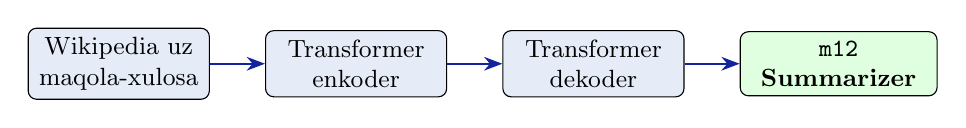
\begin{tikzpicture}[
      mod/.style={draw, fill=cnubluebg, rounded corners=3pt,
                  minimum width=2.3cm, minimum height=0.75cm,
                  font=\small, align=center},
      fin/.style={draw, fill=green!12, rounded corners=3pt,
                  minimum width=2.5cm, minimum height=0.75cm,
                  font=\small\bfseries, align=center},
      arr/.style={-{Stealth}, thick, color=cnublue}
  ]
    \node[mod] (op) {Wikipedia uz\\ maqola-xulosa};
    \node[mod, right=0.7cm of op]  (en) {Transformer\\ enkoder};
    \node[mod, right=0.7cm of en]  (de) {Transformer\\ dekoder};
    \node[fin, right=0.7cm of de]  (m12) {\texttt{m12}\\ Summarizer};
    \draw[arr] (op)--(en); \draw[arr] (en)--(de); \draw[arr] (de)--(m12);
  \end{tikzpicture}
  \end{center}
  \vspace{5pt}
  \begin{columns}[T]
    \begin{column}{0.50\textwidth}
      \textbf{P12 da qurasiz:}\\[3pt]
      \small
      \begin{itemize}\setlength\itemsep{2pt}
        \item \texttt{m12 TransformerSummarizer}: self-attention $+$ PE
        \item Wikipedia uz maqola-xulosa juftlarida o'qitish
        \item ROUGE-1 bilan baholash
      \end{itemize}
    \end{column}
    \begin{column}{0.46\textwidth}
      \textbf{Birinchi assert (bu slayd [I4]):}\\[4pt]
      \small\ttfamily
      assert abs(\\
      \phantom{xx}f1 - 0.750) < 1e-3\\[4pt]
      \normalfont\footnotesize\color{halfgray}
      \textit{\# Ma'ruza L12 [I4]-slayd bilan}\\
      \textit{\# solishtiring (ROUGE-1 F1)}
    \end{column}
  \end{columns}
\end{frame}

% ----------------------------------------------------------------
% [R] ADABIYOTLAR
% ----------------------------------------------------------------
\begin{frame}{Adabiyotlar}
  \begin{enumerate}\small\setlength\itemsep{5pt}
    \item Vaswani, A., va boshq.\ (2017). \textit{Attention Is All You Need.} NeurIPS 30.
    \item Lin, C.-Y.\ (2004). \textit{ROUGE: A Package for Automatic Evaluation
          of Summaries.} ACL Workshop.
    \item Devlin, J., va boshq.\ (2019). \textit{BERT: Pre-training of Deep
          Bidirectional Transformers.} NAACL-HLT 2019.
    \item Raffel, C., va boshq.\ (2020). \textit{Exploring the Limits of Transfer
          Learning with a Unified Text-to-Text Transformer (T5).} JMLR 21.
    \item \texttt{torch.nn.Transformer} va \texttt{rouge\_score} hujjatlari.
  \end{enumerate}
\end{frame}

% ================================================================
% [S] ILOVALAR (appendix --- slayd soniga kirmaydi)
% ================================================================
\appendix

\begin{frame}{Ilova S1: multi-head attention to'liq matematikasi}
  \small
  $h$ ta head, har biri $d_k=d/h$ o'lchamli:
  $$ \mathrm{head}_i = \mathrm{softmax}\!\left(\frac{(XW_i^Q)(XW_i^K)^{\top}}{\sqrt{d_k}}\right)(XW_i^V) $$
  \bunda{$W_i^Q, W_i^K, W_i^V \in \mathbb{R}^{d\times d_k}$ --- har head
  proyeksiyalari; natijalar konkatenatsiya qilinib $W^O \in \mathbb{R}^{d\times d}$
  bilan birlashtiriladi.}
  \vspace{4pt}

  Har head turli munosabatni o'rganadi; $d_k=d/h$ tanlovi umumiy hisobni bitta
  to'liq o'lchamli attention bilan teng saqlaydi.
\end{frame}

\begin{frame}{Ilova S2: ROUGE-L (eng uzun umumiy ketma-ketlik)}
  \small
  ROUGE-L unigram emas, \textbf{LCS} (longest common subsequence) ga asoslanadi:
  $$ R_{lcs} = \frac{\mathrm{LCS}(X,Y)}{|Y|}, \qquad
     P_{lcs} = \frac{\mathrm{LCS}(X,Y)}{|X|}, \qquad
     F_{lcs} = \frac{2 P_{lcs} R_{lcs}}{P_{lcs}+R_{lcs}} $$
  \bunda{$X$ --- hypothesis, $Y$ --- reference; $\mathrm{LCS}$ --- tartibni
  saqlagan eng uzun umumiy ketma-ketlik uzunligi.}
  \vspace{4pt}

  Misol: $X=$\texttt{nlp juda foydali}, $Y=$\texttt{nlp juda qiziq va foydali}
  $\Rightarrow$ LCS $=$ \texttt{nlp juda foydali} (uzunligi 3, tartib saqlangan).
\end{frame}

\end{document}
